\documentclass[a4paper, 12pt]{report}
\usepackage{graphicx}
\usepackage[french]{babel}
\usepackage[utf8]{inputenc}
\usepackage[T1]{fontenc}
\usepackage{multirow}
\usepackage{listings}
\usepackage{float}
\usepackage[french]{babel}
\usepackage[breaklinks]{hyperref}
\usepackage{subcaption}
\captionsetup{compatibility=false}
\hypersetup{pageanchor=false}


\begin{document}

\begin{titlepage}
  \begin{center}
    \begin{tabular*}{\textwidth}{l@{\extracolsep{\fill}}r}
      
\includegraphics[height=1.5cm]{images/m1info.eps}&
			
\includegraphics[height=1.5cm]{images/P8.eps}
    \end{tabular*}
    \small 
    \rule{\textwidth}{.5pt}~\\
    \large 
    \textsc{Université Paris 8 - Vincennes à Saint-Denis}\vspace{0.5cm}\\
    \textbf{Master Informatique}\vspace{3.0cm}\\
    \Large
    \textbf{Rapport de projet tuteuré}\vspace{1.5cm}\\
    \large
    \textbf{Samuel \textsc{de Vals}}\\
		\textbf{Paul \textsc{Vialart}}\vspace{1.5cm}\\
    Date de soutenance : le 15/06/2018\vspace{1.75cm}\\
  \end{center}\vspace{1.5cm}~\\
  \begin{tabular}{ll}
    \hspace{-0.45cm}Tuteur -- Université~:~&~Sylvia \textsc{Chalençon}
  \end{tabular}
\end{titlepage}

\newpage\null\newpage

\chapter*{Résumé}
\markboth{\sc Résumé}{}
\addcontentsline{toc}{chapter}{Résumé} 
TODO: Résumé du projet et des tâches accomplies

\chapter*{Introduction}
\markboth{\sc Introduction}{}
\addcontentsline{toc}{chapter}{Introduction}
\input{teX/001_introduction.tex}

%adding content into the summary page /!\ need 2 compilations
\tableofcontents

\chapter*{Le choix de l'API three.JS}
\markboth{\sc Le choix de l'API three.JS}{}
\addcontentsline{toc}{chapter}{Le choix de l'API three.JS}
Nous avons tout d'abord découpé le projet en différentes tâches à réaliser afin de le mener à son terme. Voici un schéma représentant les principales étapes d'élaboration du projet.

\begin{center}
	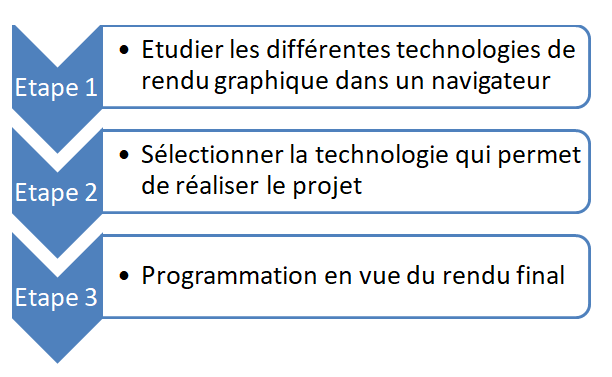
\includegraphics[height=7cm]{images/Processus_DEV.png}\\
	\textit{Processus de développement utilisé au cours du projet}\\
\end{center}

\newpage
Pour ce projet, nous avons choisi l'API three.JS. Celle-ci permet de faire du WebGL de façon simple et facilite la mise en œuvre du projet. En effet, ce projet est notre premier contact avec le domaine du WebGL. Avec sa communauté active, ses nombreux tutoriels et ses exemples détaillés, three.JS semble être la méthode la plus simple pour modéliser l'environnement qui nous a été demandé.

Cette API permet de simuler une vaste variété de rendus en 3D paramétrables. Il peut s'agir de décors, de personnages, d'effets de particules, etc.

\begin{center}
	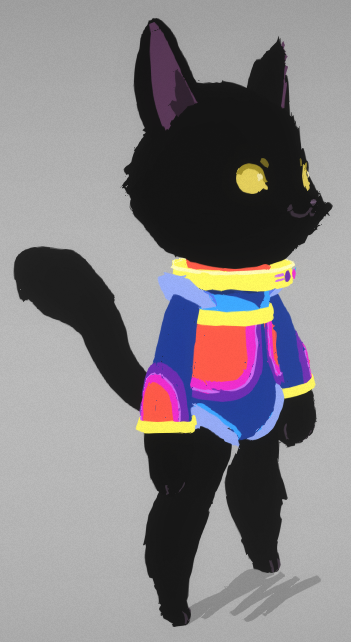
\includegraphics[height=6cm]{images/threeJS_poly_cat.png}\\
	\textit{Exemple de personnage 3D généré avec le module Poly de three.JS}
\end{center}

\begin{center}
	
\includegraphics[height=6cm]{images/threeJS_poly_particle.png}\\
	\textit{three.JS permet également de reproduire des effets de particules avancés...}
\end{center}

\begin{center}
	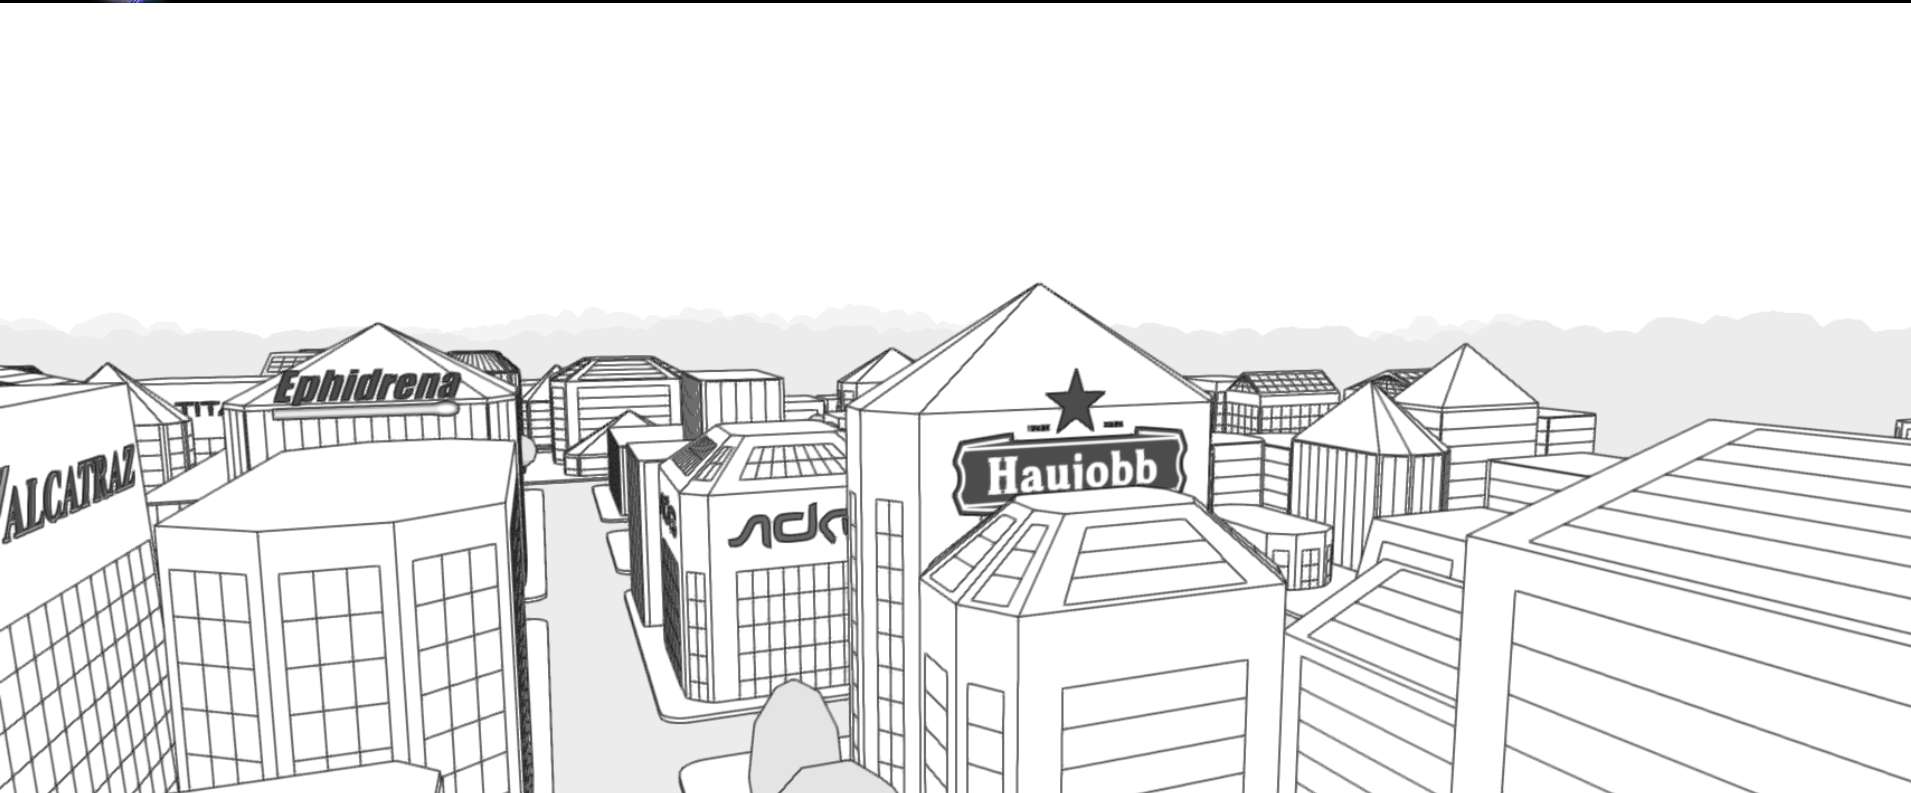
\includegraphics[height=6cm]{images/threeJS_poly_city.png}\\
	\textit{... voire des villes entières.}
\end{center}



Dans notre cas, la page web génère un monde virtuel avec le bruit de Perlin. Afin de partir sur une modélisation cubique, proche du rendu final en style Lego, nous nous sommes orientés vers une déclinaison de l'API reproduisant l'univers du jeu vidéo Minecraft, réputé pour son univers tout en cubes. Voici le rendu graphique de l'exemple :

\begin{center}
	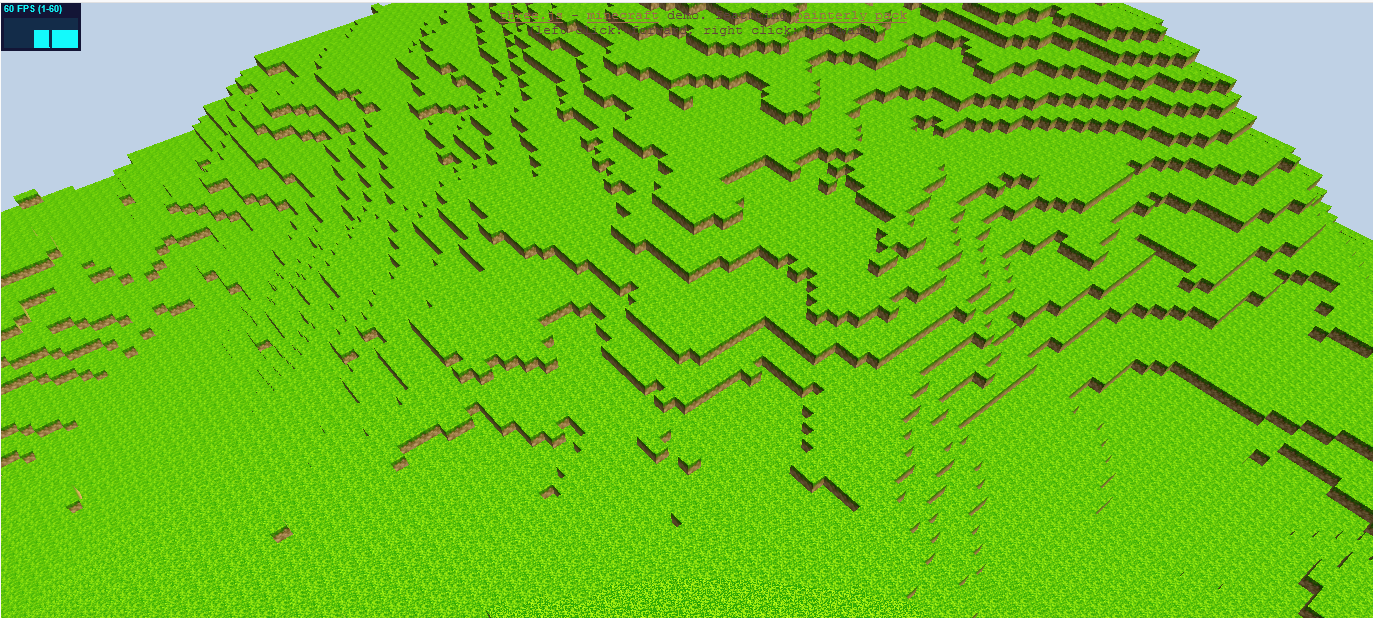
\includegraphics[height=6cm]{images/threeJS_minecraft.png}\\
	\textit{Exemple du monde virtuel généré avec l'API three.JS}
	\footnote{Le code source de l'exemple de l'API three.JS se trouve là : \url{https://github.com/mrdoob/three.js/blob/master/examples/webgl_geometry_minecraft.html}}
\end{center}

Il a ensuite fallu adapter le projet afin de mettre le code source HTML, CSS, et JS dans des fichiers séparés.

\begin{center}
	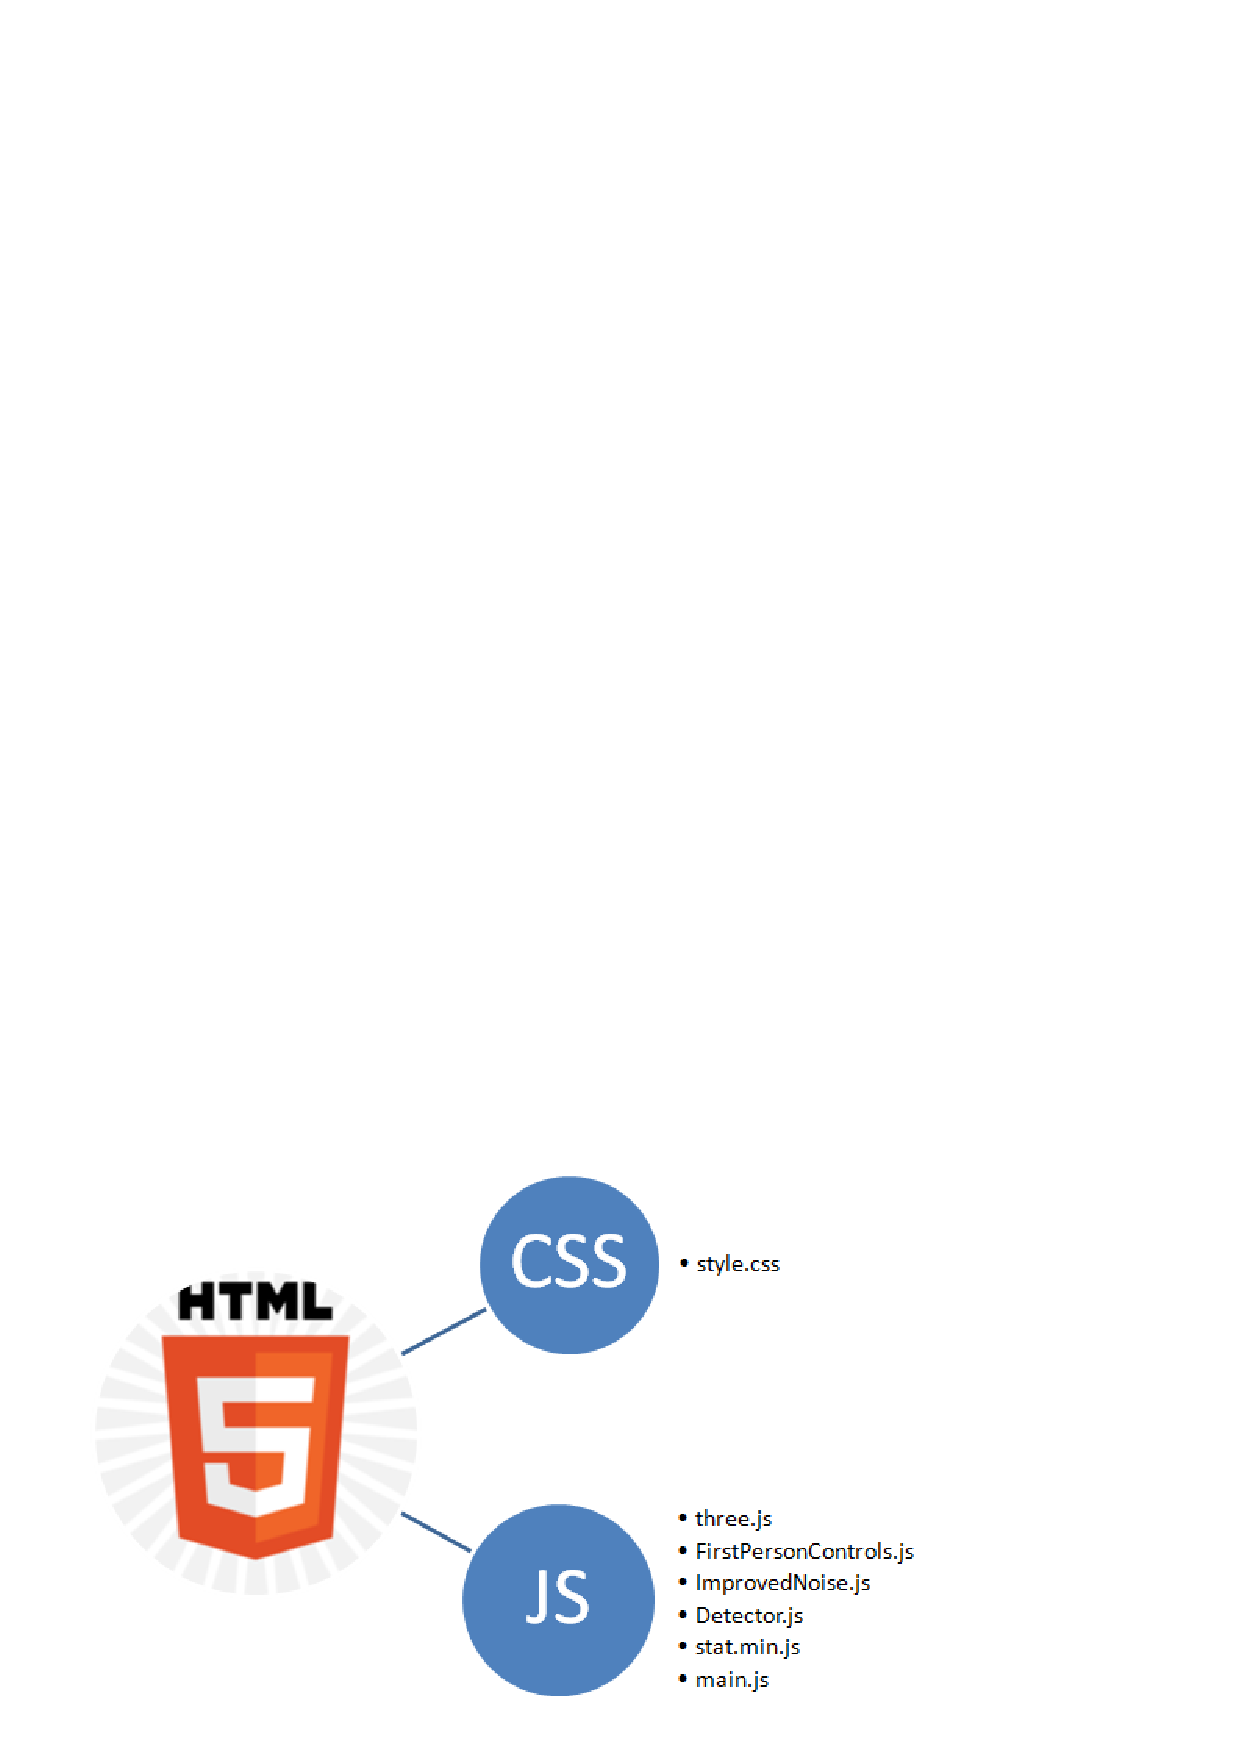
\includegraphics[height=6cm]{images/ProFileOrganisation.png}\\
	\textit{Structure du projet}
\end{center}

\chapter*{Le bruit de Perlin}
\markboth{\sc Le bruit de Perlin}{}
\addcontentsline{toc}{chapter}{Le bruit de Perlin}
Le bruit de Perlin est très utilisé dans la génération d'image. Effet, ce bruit permet de déterminer une élévation d'un sommet de N-dimension (dans notre cas 3). Nous avons donc implémenté un algorithme de afin de générer. L'algorithme se divise en deux temps :

\begin{enumerate}
	\item Initialisation
	\item Calcul
\end{enumerate}

La phase d'initialisation consite à avoir un tableau de 512 éléments bien mélangés compris entre 0 et 255. Enfin, le tableau se répète à partir de la valeur 256 (tab[0] = tab[256], et ainsi de suite). La phase de calcul est plus compliquée, car elle se découpe en plusieurs étapes. Le principe de l'algorithme est de retourner une même valeur en fonction d'un x, d'un y, et d'un z donné. On place x, y , z dans l'interval [0;255] avec un "et" logique. Ensuite on calcul les coordonnées en gradient du cube dans l'espace. Enfin, on calcul la valeur de retour. Ken Perlin a ensuite amélioré cet algorithme, afin qu'il soit plus performant en terme de calcul et de résultat. Cette version s'appelle le bruit de simplex.

Afin de générer aléatoirement un monde virtuel, il est necessaire de remplir le tableau aléatoirement à chaque démarrage du projet. En effet, sinon on obtiendra toujours la même monde carte, car le tableau de permutation reste toujours le même entre deux chargements.



\chapter*{Les améliorations réalisées}
\markboth{\sc Les améliorations réalisées}{}
\addcontentsline{toc}{chapter}{Les améliorations réalisée}
\section{L'aspect visuel}

Parmi les points d'amélioration figurait le \texttt{rendu de la carte}. Pour rappel, voici a quoi elle ressemblait lors de la premiere version :

\begin{center}
	\null\vspace{0.25cm}
	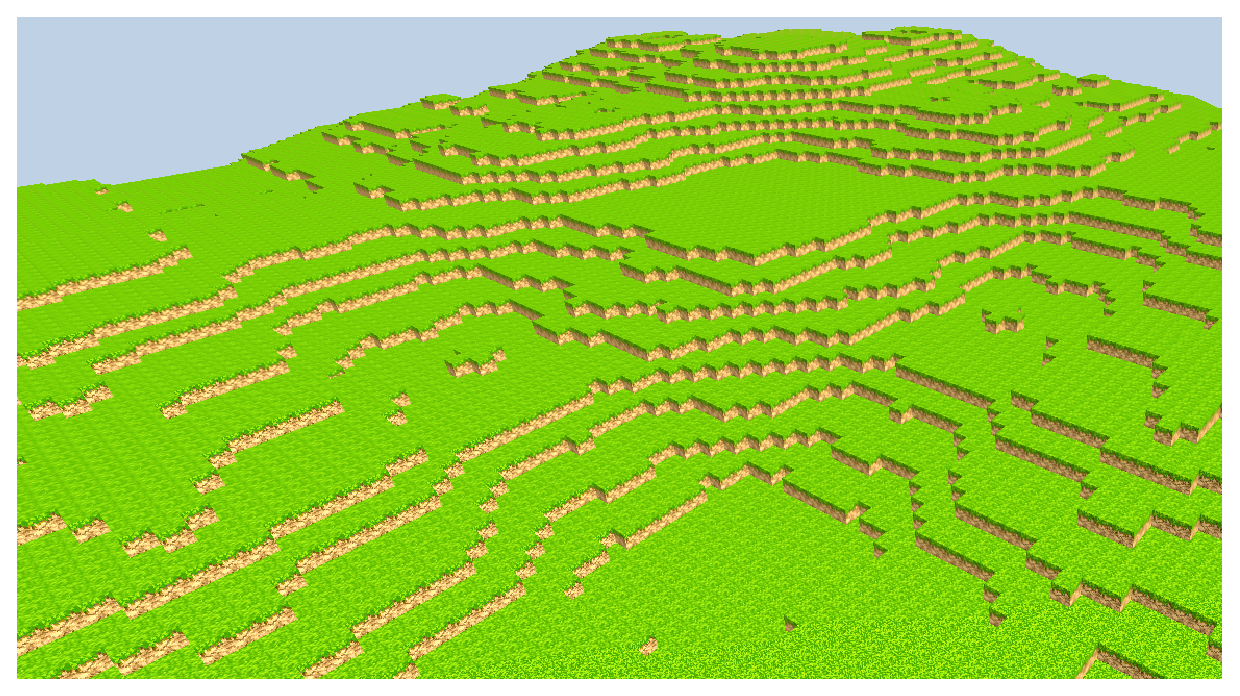
\includegraphics[height=3cm]{images/OurMinecraftWorld.eps}\\
	\textit{Image 9. Ancienne carte.}\\
\end{center}

Cette carte a depuis subi de nombreuses améliorations, tant visuelles que du point de vue de la jouabilité. En effet, lors de la dernière version de ce projet (que nous appellerons V0), nous clôturions le rapport avec une liste d'axes d'améliorations. Nous n'avons eu qu'à piocher dans cette liste au gré des envies afin d'agrémenter le projet de nouveautés, et ainsi lui faire adopter la forme qu'il possède à l'heure actuelle.

\begin{center}
	\null\vspace{0.25cm}
	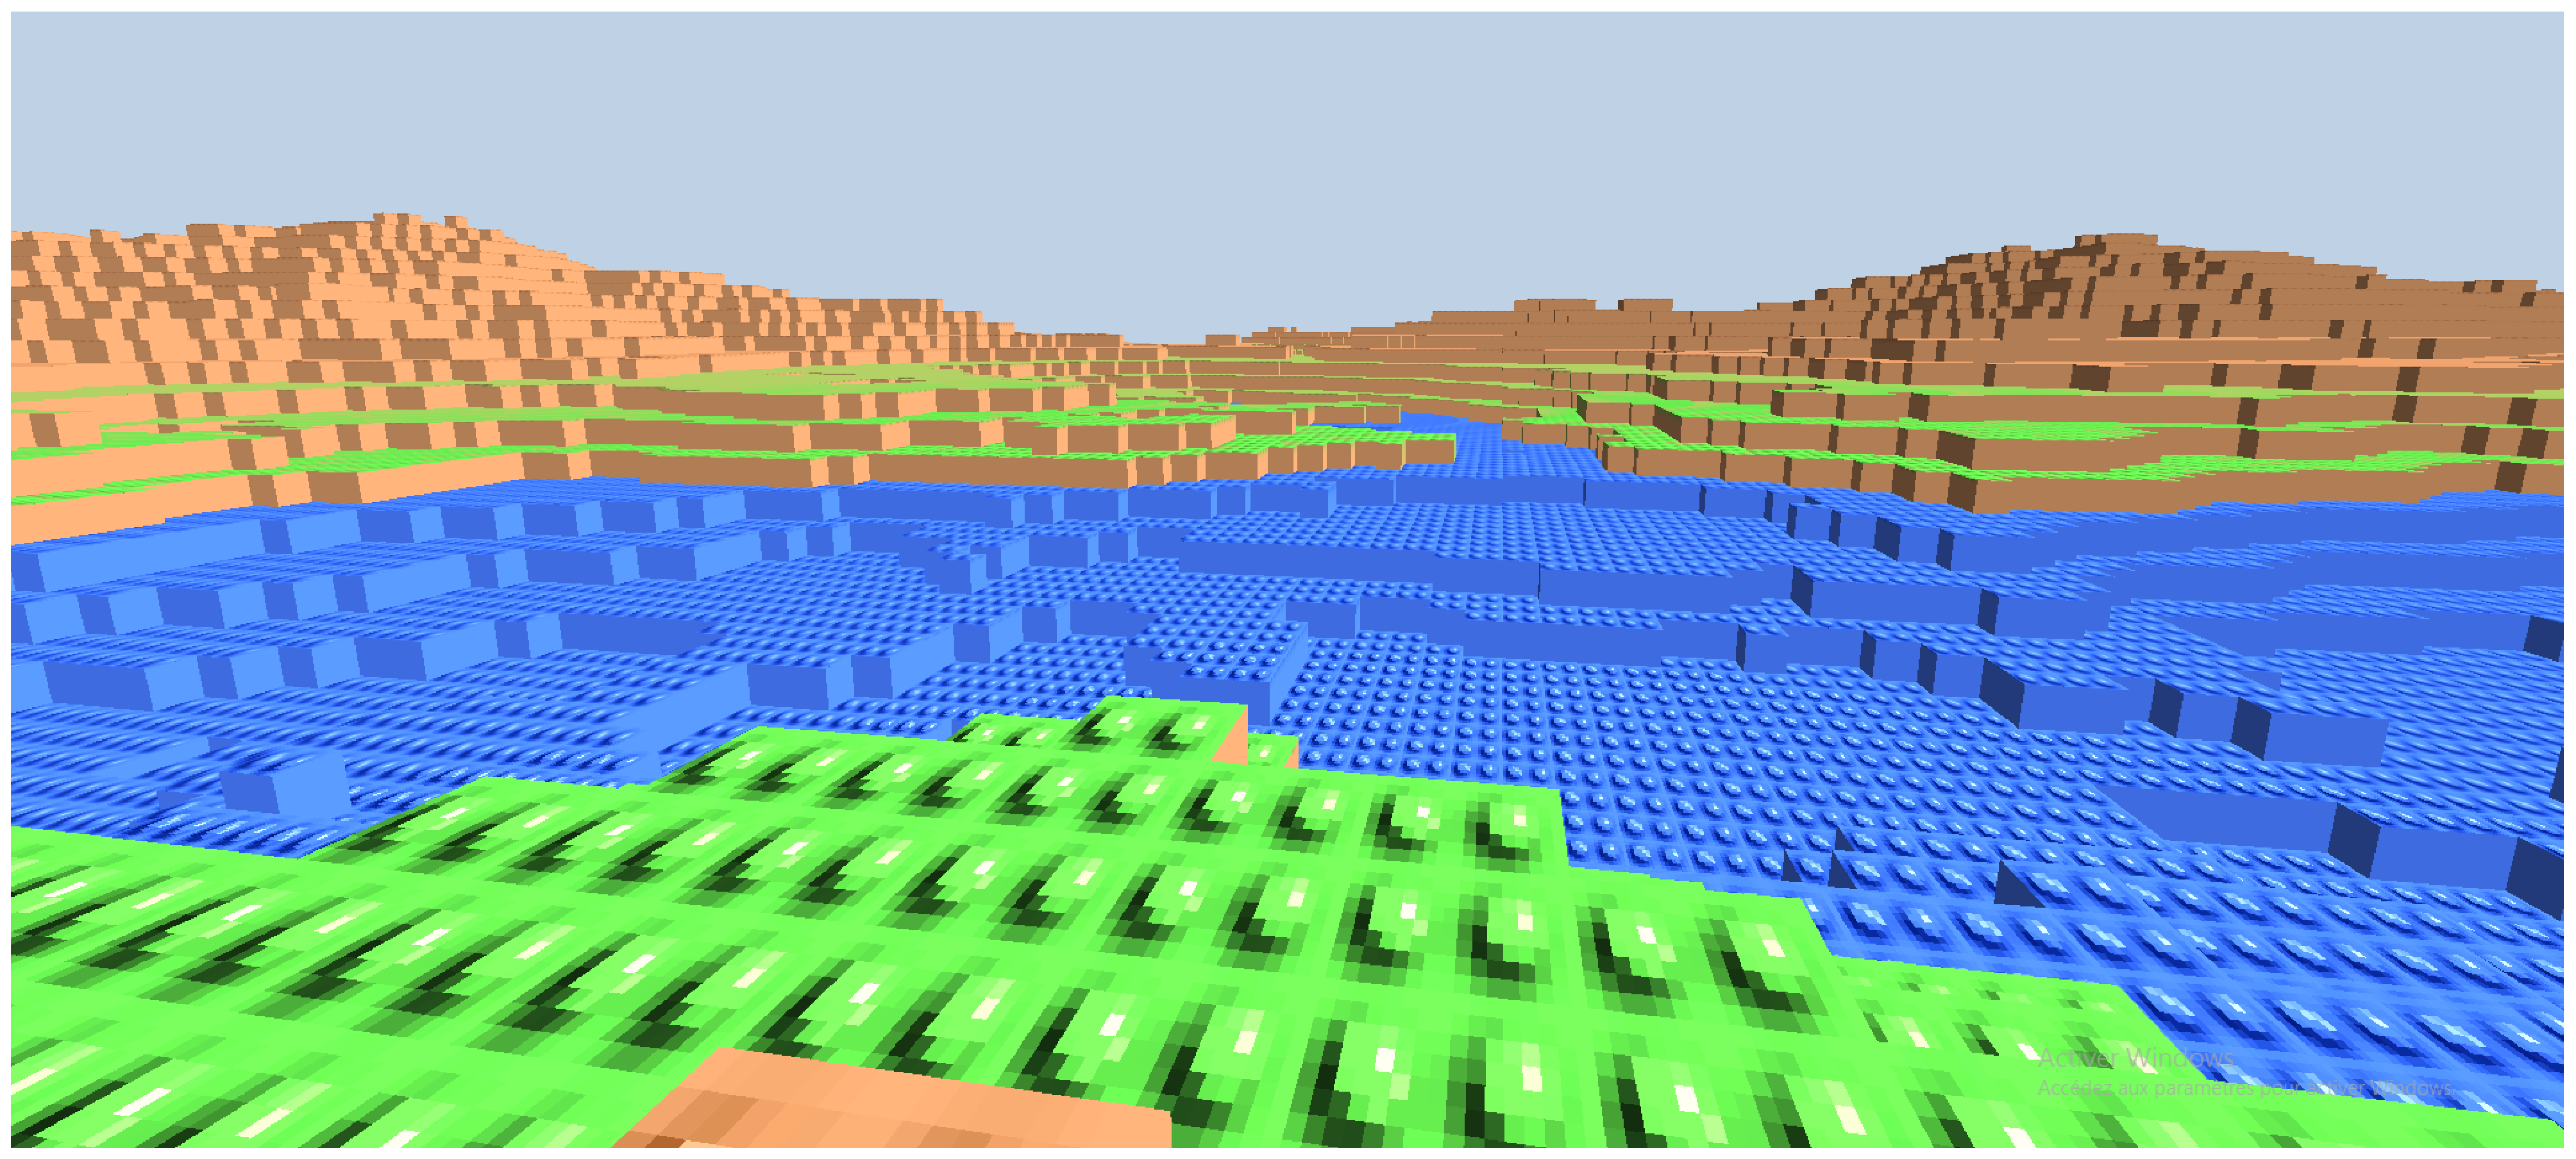
\includegraphics[height=3cm]{images/newworld4.eps}\\
	\textit{Image 10. Nouvelle carte.}\\
\end{center}

Afin d'adopter un rendu visuellement plus proche de ce que nous recherchions, la fabrication de la carte a connu deux ajouts :
\begin{enumerate}
	\item \textbf{Nouvelles textures.}
	\item \textbf{Changement de textures.}
\end{enumerate}

Puisque nous cherchions un rendu visuel proche de Lego et que l'API Three.JS s'inspire de Minecraft, nous avons choisi un pack de textures Minecraft, LegoPack. 
 
\begin{center}
	
\includegraphics[height=3cm]{images/grass.eps}\\	
\includegraphics[height=3cm]{images/dirt.eps}\\	
\includegraphics[height=3cm]{images/water.eps}\\
	\textit{Image 11. Aperçu des nouvelles textures.}\\
\end{center}

Ces nouvelles textures remplacent l'ancienne texture unique et uniforme. Puis, afin d'appliquer un peu de variété au relief et d'exploiter au mieux les nouvelles textures, nous avons établi trois niveaux de terrain lors de la génération de la carte par le bruit de Perlin :
\begin{enumerate}
	\item \textbf{La montagne (Hight Layer)}
	\item \textbf{La prairie (Middle Layer)}
	\item \textbf{La mer (Low Layer)}
\end{enumerate}
Le type de terrain varie en fonction de la hauteur de celui-ci. Pour ce faire, lors du calcul initial de la carte, on récupère la hauteur de chaque bloc et on lui applique une texture en fonction de cette valeur.

\begin{center}
	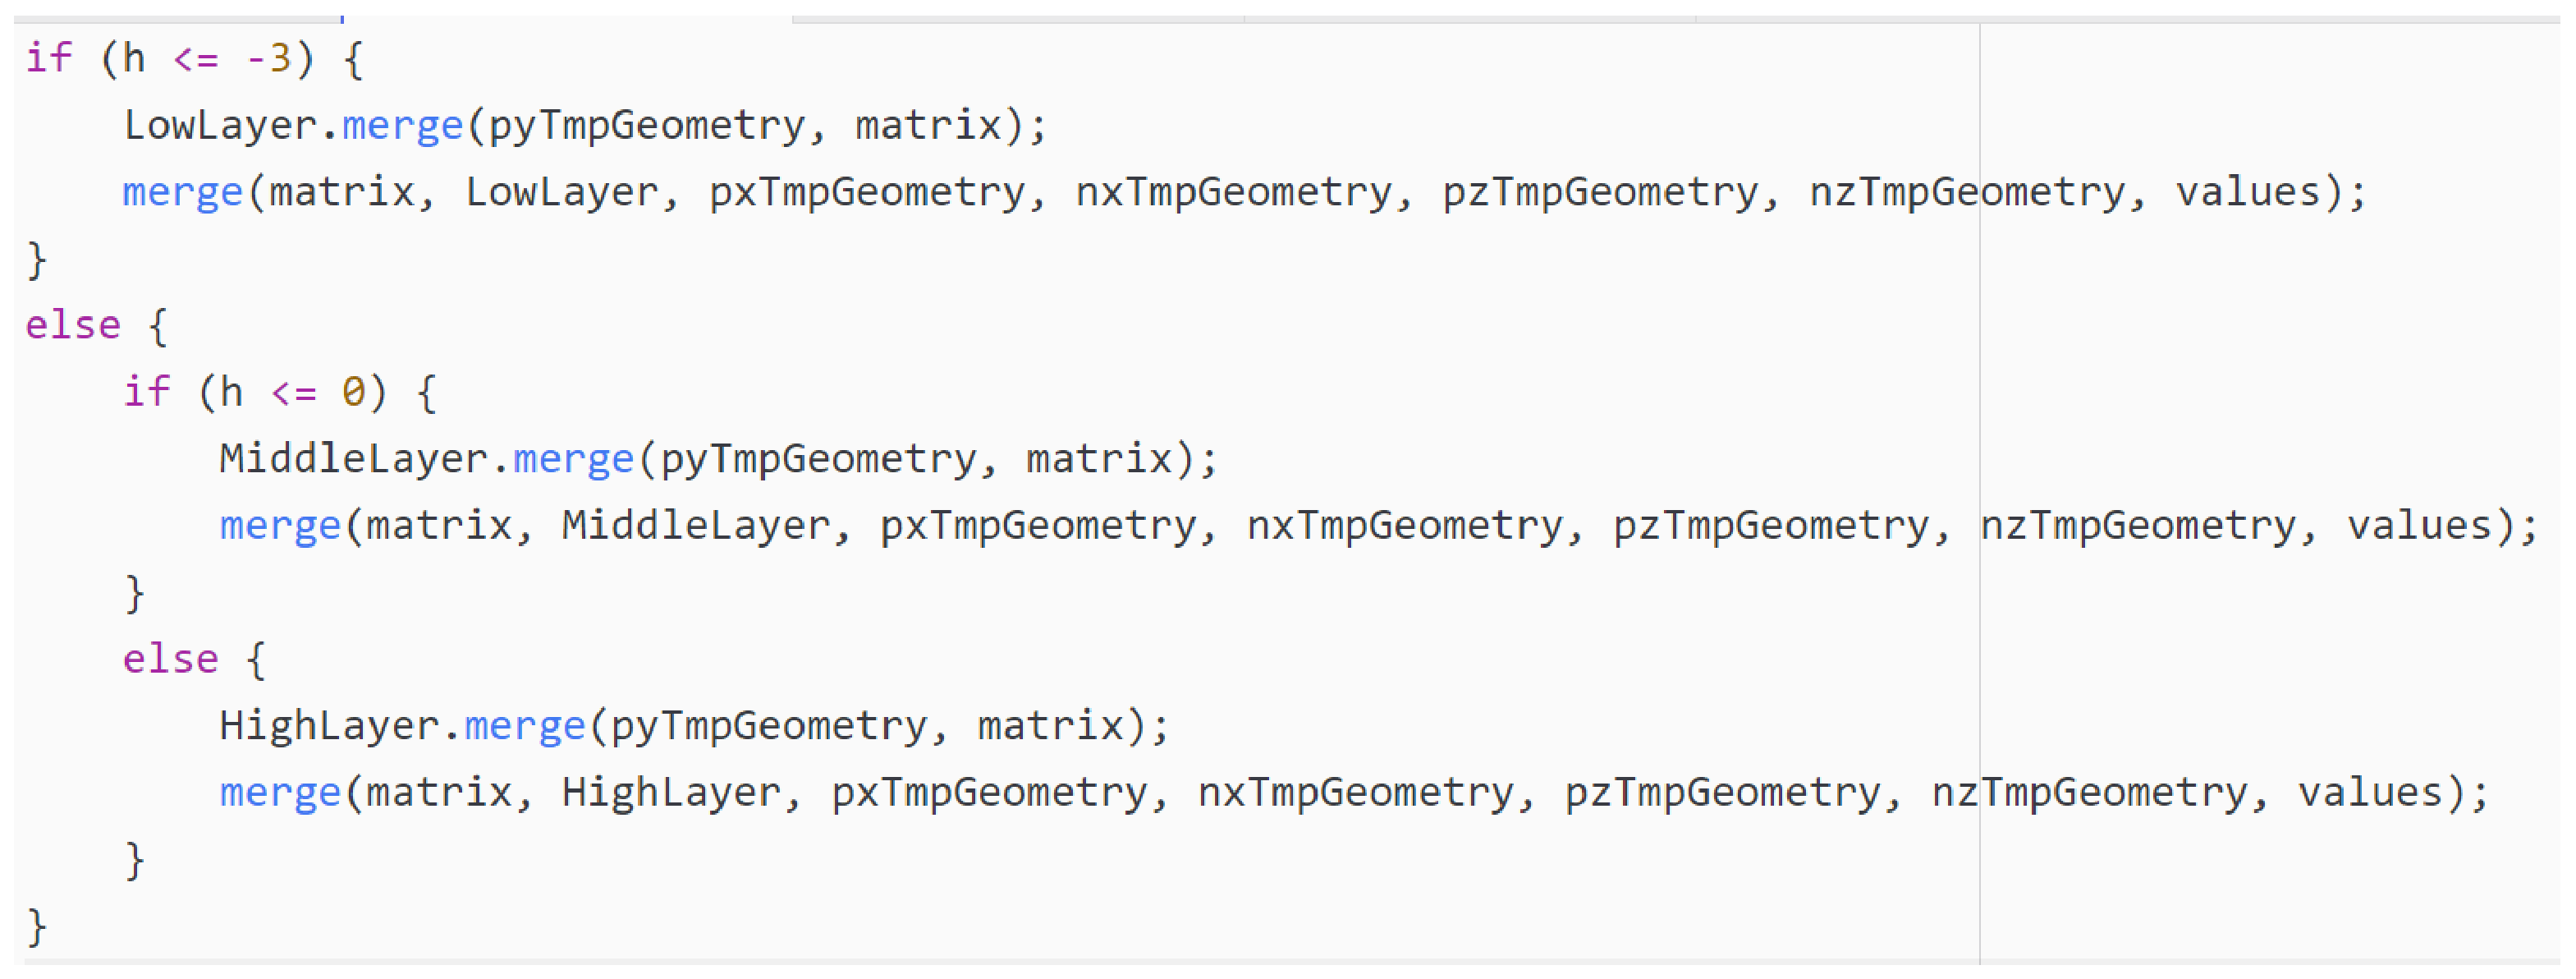
\includegraphics[height=3cm]{images/code_cubes.eps}\\	
	\textit{Extrait de code 1. En fonction de la hauteur du cube, on lui applique une texture différente.}
\end{center}


\section{La physique du terrain}
Par défaut, l'ancienne version de la carte ne possédait pas de physique : la caméra pouvait voler dans toutes les directions et même passer à travers la carte. Désormais, le personnage ne peut se déplacer que sur le sol. 
Désormais, le sol possède une physique et le personnage ne peut pas le traverser. Pour ce faire, il a fallu ajouter un contrôle de la hauteur de la caméra par rapport au cube qu'il est en train de parcourir, et de recalculer sa hauteur en fonction de celle des cubes au sol. 

\begin{center}
	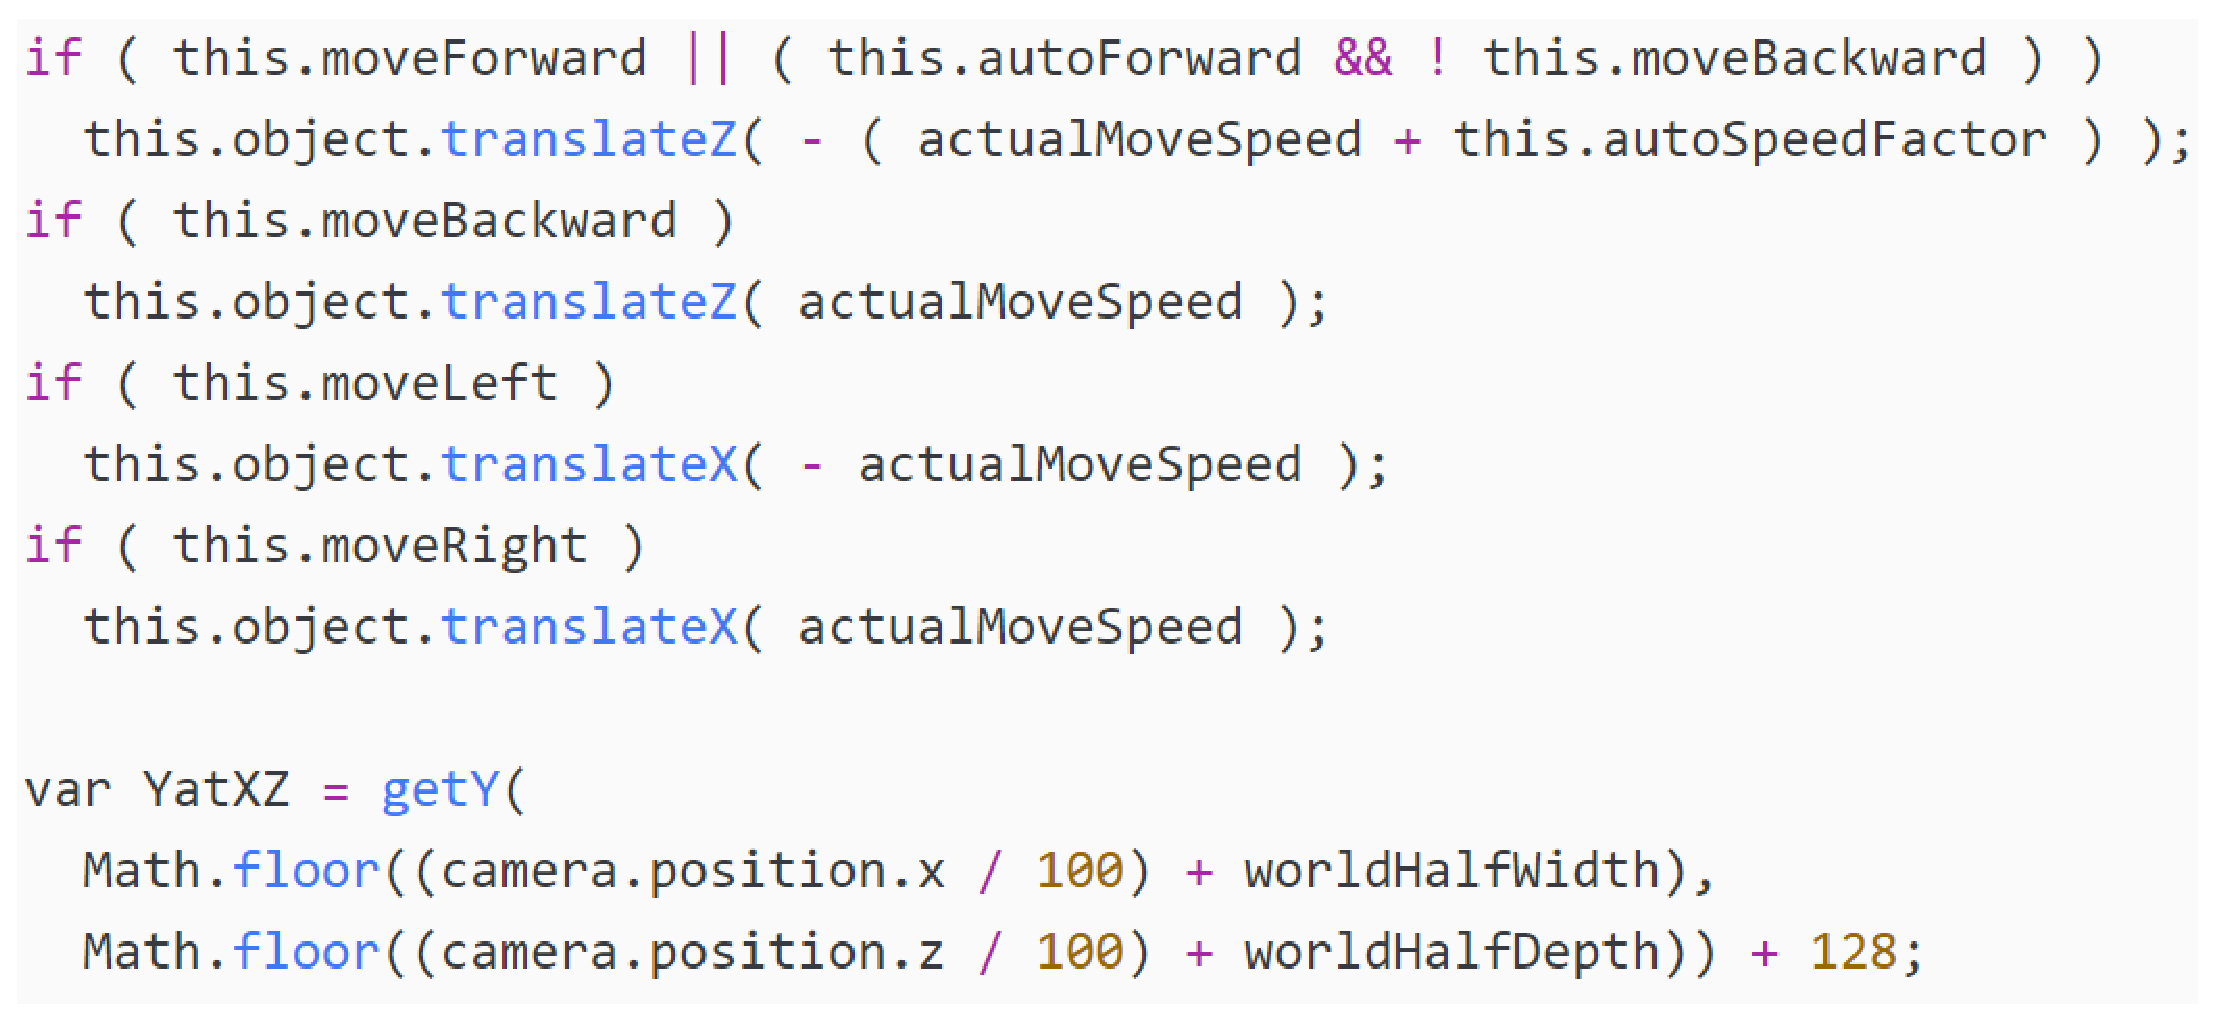
\includegraphics[height=3cm]{images/code_hauteur.eps}\\
	\textit{Extrait de code 2. Gestion de la hauteur du personnage en fonction de sa position à l'intérieur de l'environnement.}
\end{center}


\section{Les contrôles}
L'unde des exigences de la nouvelle version était de refaire les contrôles du jeu. En effet, three.js était par défaut configurée en QWERTY, ce qui rendait les contrôles complexes sur un clavier en AZERTY.
Il faut savoir que dans three.JS, les contrôles sont localisés dans un objet nommé FirstPersonControls. Initialisé pendant la phase de génération du monde, cet objet vérifie les entrées utilisateur et les compare avec une liste d'événements. Les plus importants de ces événements sont onMouseMove (pour calculer la rotation de la caméra), onMouseDown et onMouseUp (quand un clic de la souris est enfoncé puis relâché) et onKeyDown et onKeyUp (même chose pour le clavier.) Lorsque l'un de ces événements survient, le programme récupère le code de la touche enfoncée afin de vérifier si elle correspond à une action.

\begin{center}
	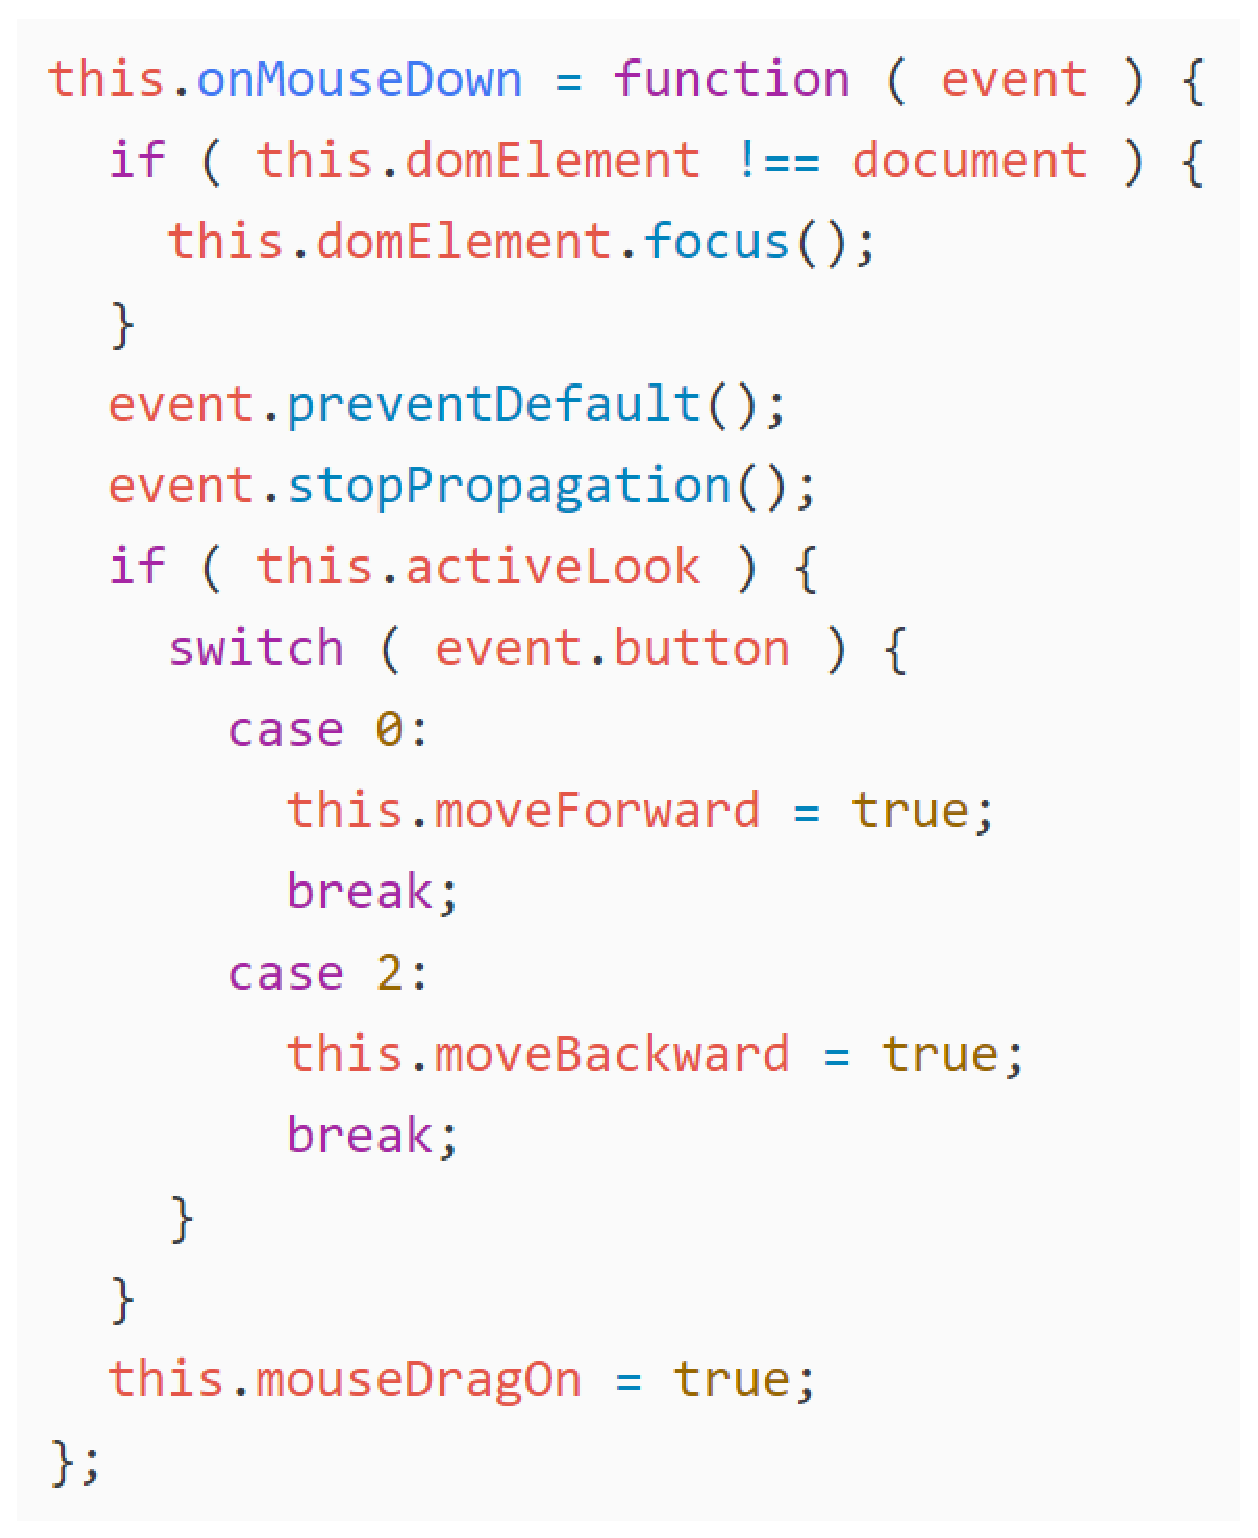
\includegraphics[height=3cm]{images/code_onmousedown.eps}\\
	\textit{Extrait de code 3. Gestion du clic de la souris avec l'événement onMouseDown.}
\end{center}

\chapter*{Les axes d'amélioration}
\markboth{\sc Les axes d'amélioration}{}
\addcontentsline{toc}{chapter}{Les axes d'amélioration}
Une fois parvenus au terme de cette V1, nous avons donc réalisé la plupart des améliorations que nous avions prévues. Voici cependant celles que nous n'avons pas pu faire :

\vspace{0.5cm}
\begin{enumerate}
	\item \textbf{Rendre le personnage visible} : L'intérêt du projet est également de représenter un personnage évoluant dans l'univers généré. Son apparence reste encore à décider.
	\item \textbf{Implémenter génération de terrain avec le bruit de Simplex }: Le bruit de Simplex étant la version évoluée et plus moderne du bruit de Perlin, il serait intéressant de se pencher dessus afin de saisir les différences entre ces deux algorithmes, et d'observer le résultat sur notre carte en 3D. 
	\item \textbf{Ajouter divers éléments de décors }(arbres, cours d'eau, etc.) : Y ajouter des éléments ponctuels lui donnerait un peu plus de vie et de réalisme.
\end{enumerate}








\chapter*{Conclusion}
\markboth{\sc Conclusion}{}
\addcontentsline{toc}{chapter}{Conclusion}
En guise de conclusion, on peut dire que ce projet aura été instructif sur X points :
\vspace{0.5cm}
\begin{enumerate}
	\item \textbf{Le LateX} : ce langage représente encore une petite difficulté puisque la conception (et non la rédaction) de ce rapport aura été semé d'embûches. Mais nous aurons tout de même appris à nous servir de cette technologie, ce qui s'avèrera sans doute utile plus tard dans le cadre de nos futurs travaux de recherche ou de nos projets professionnels.
	\item \textbf{Three.JS} : cette API demeure un outil puissant, parfois un peu complexe d'utilisation au premier abord, mais riche en paramètres et en possibilités. Si nous ne prétendons pas maîtriser Three.JS à l'issue de ce projet, nous nous contentons tout de même d'être capables de reproduire des environnements WebGL avec un peu d'efforts et d'investissement pour explorer la très riche documentation de cette API.
	\item \textbf{Le bruit de Perlin} : cet algorithme, ou du moins sa version améliorée, demeure au coeur de nombreux travaux aujourd'hui, dans la recherche ou les grandes industries de divertissemement. Il était donc intéressant d'avoir une vue de l'intérieur et d'étudier le fonctionnement de cette algorithme, que nous recroiserons probablement au cours de notre parcours informatique.
\end{enumerate}

La découverte des technologies tel que le webGL, et la rédaction de document en lateX a été très enrichissante. En effet, nous avons pu rapidement voir ce qu'il était possible de faire en webGL à travers l' API three.JS qui propose un large panel d'exemple. De plus, nous avons pu étudier le fonctionnement de l'algorithme de génération de bruit de Perlin qui est très utilisé dans le monde de génération procédurale de terrain. Cependant, il nous reste encore beaucoup à faire pour terminer ce projet.



\chapter*{Références}
\markboth{\sc Références}{}
\addcontentsline{toc}{chapter}{Références}

\vspace{0.5cm}
Nick Pettit. \textit{The Begennier's Guide to three.js}. \href{http://blog.teamtreehouse.com/the-beginners-guide-to-three-js}{Team Treehouse}. 2013.

\vspace{0.5cm}
Ken Perlin. \textit{Improved Noise reference implmentation.} \href{http://mrl.nyu.edu/~perlin/noise/}{New York University Media Research Lab}. 2002.

\vspace{0.5cm}
Adrian Biagioli. \textit{Understanding Perlin Noise.} \href{https://flafla2.github.io/2014/08/09/perlinnoise.html}{Adrian's Soapbox}. 2014.

\vspace{0.5cm}
Herman Tulleken. \textit{How to use Perlin Noise in your games.} \href{http://devmag.org.za/2009/04/25/perlin-noise/}{Dev.Mag}. 2009.

\vspace{0.5cm}
Stefan Gustavson. \textit{Simplex Noise demystified.} \href{http://staffwww.itn.liu.se/~stegu/simplexnoise/simplexnoise.pdf}{Linköping University}. 2005.



\end{document}